\subsubsection{Optimisation for Deep Learning}

\begin{remark} \hlt{Optimisation}\\
A cost function $J(\bm{\theta})$ is reduced to improve some performance measure $P$.\\
Optimisation algorithms include some specialisation on specific structure of machine learning objective functions.\\
Cost function is average over training set,
\begin{equation}
J(\bm{\theta}) = \mathbb{E}_{(\bm{x}, y) \sim \hat{p}_{\text{data}}} L(f(\bm{x}; \bm{\theta}), y) \nonumber
\end{equation}
where $L$ is per-example loss function, $f(\bm{x}; \bm{\theta})$ is predicted output given input $\bm{x}$, $\hat{p}_{\text{data}}$ is empirical distribution. For supervised learning, $y$ is target output.\\
The goal is to usually to minimise objective function where expectation is taken on data generating distribution $p_{\text{data}}$ rather than over the finite training set:
\begin{equation}
J^*(\bm{\theta}) = \mathbb{E}_{(\bm{x}, y) \sim p_{\text{data}}} L(f(\bm{x}; \bm{\theta}), y) \nonumber
\end{equation}
Note that machine learning algorithm usually minimises a surrogate loss function, and halts when convergence criterion based on early  stopping is satisfied.
\end{remark}

\begin{definition} \hlt{Empirical Risk Minimisation}\\
To minimise expected loss on training set, where $\hat{p}(\bm{x}, y)$ is the empirical distribution. The empirical risk is
\begin{equation}
\mathbb{E}_{\bm{x}, y \sim \hat{p}_{\text{data}}(\bm{x}, y)}[L(f(\bm{x}, \bm{\theta}), y)] = \frac{1}{m} \sum\limits_{i=1}^m L(f(\bm{x}^{(i)}; \bm{\theta}), y^{(i)}) \nonumber
\end{equation}
where $m$ is number of training samples. Note that empirical risk minimisation is prone to overfitting, as models with high capacity may memorise the training set.
\end{definition}

\begin{remark} \hlt{Batch and Minibatch Algorithms}\\
Objective algorithms for machine learning computes each update to the parameters based on expected value of cost function using only a subset of terms of full cost function.\\
For maximum likelihood estimation problems, note that
\begin{align}
\bm{\theta}_{\text{ML}} &= \arg \max_{\bm{\theta}} \sum\limits_{i=1}^m \log p_{\text{model}}(\bm{x}^{(i)}, y^{(i)}; \bm{\theta}) \nonumber \\
J(\bm{\theta}) &= \mathbb{E}_{\bm{x}, y \sim \hat{p}_{\text{data}}} \log p_{\text{model}} (\bm{x}, y; \bm{\theta}) \nonumber
\end{align}
The gradient is then
\begin{equation}
\nabla_{\bm{\theta}} J(\bm{\theta}) = \mathbb{E}_{\bm{x}, y \sim \hat{p}_{\text{data}}} \nabla_{\bm{\theta}} \log \log p_{\text{model}} (\bm{x}, y; \bm{\theta}) \nonumber
\end{equation}
If the optimisation algorithm uses the entire training set, then it is a batch gradient method.\\
If a single sample is used at a time, then this is a stochastic/online gradient method.\\
For algorithms that uses more than one but less than all samples, then this is a minibatch gradient method.
\end{remark}

\begin{remark} \hlt{Challenges: Ill-Conditioning of Hessian Matrix $H$}\\
May cause stochastic gradient descent to be stuck where very small step increases the cost function.\\
Note that a gradient descent step of $- \bm{\epsilon} \bm{g}$ will add
\begin{equation}
\frac{1}{2} \epsilon^2 \bm{g}^T \bm{H} \bm{g} - \epsilon \bm{g}^T \bm{g} \nonumber
\end{equation}
to the cost. This will be a problem when $\frac{1}{2} \epsilon^2 \bm{g}^T \bm{H} \bm{g} > \epsilon \bm{g}^T \bm{g}$.\\
Monitor squared gradient norm $\bm{g}^T \bm{g}$ and $\bm{g}^T \bm{H} \bm{g}$ term. When ill-conditioning happens, gradient norm does not shrink significantly but $\bm{g}^T \bm{H} \bm{g}$ term grows more than order of magnitude, and learning rate shrinks.
\end{remark}

\begin{remark} \hlt{Challenges: Local Minimums}\\
Model is identifiable if a sufficiently large training set can rule out all but one setting of model parameters.\\
There may be an extremely large or uncountably infinite amount of local minima in a cost function. If the local minima have a high cost compared to global minimum, then this is problematic.
\end{remark}

\begin{remark} \hlt{Challenges: Plateaus, Saddle Points, Flat Regions}\\
For a function $f: \R^n \rightarrow \R$, expected ratio of saddle points to local minima grows exponentially with $n$. Hessian matrix at a saddle point has a mixture of positive and negative eigenvalues.\\
Degenerate regions with flat gradient may correspond to high value of objective function.
\end{remark}

\begin{remark} \hlt{Challenges: Cliffs and Exploding Gradients}\\
On extremely steep cliff structure, gradient update step may move parameters extremely far, losing most of the optimisation work done previously. The consequences may be mitigated using gradient clipping heuristics, which reduces the step size to be small enough.
\end{remark}

\begin{remark} \hlt{Challenges: Long-Term Dependencies}\\
Occurs when computational graph becomes very deep. Let a computational graph contain a path that repeatedly multiply a matrix $\bm{W}$. After $t$ steps, this is $\bm{W}^t$. Let the eigen-decomposition of $\bm{W}$ be $\bm{W} = \bm{V} \text{diag}(\bm{\lambda}) \bm{V}^{-1}$. Then we can see that $\bm{W}^t = (\bm{V} \text{diag}(\bm{\lambda}) \bm{V}^{-1})^t = \bm{V} \text{diag}(\lambda)^t \bm{V}^{-1}$.\\
There will be a vanishing and exploding gradient problem if gradients on the graph are scaled according to $\text{diag}(\bm{\lambda})^t$.  Note that recurrent networks uses same $\bm{W}$ at each time step, hence may face the problem.
\end{remark}

\begin{remark} \hlt{Stochastic Gradient Descent (SGD)}\\
Crucial parameter is the learning rate, which may be changed over time; at iteration $k$ this is $\epsilon_k$.\\
The SGD gradient estimation introduces a source of noise that does not vanish even at minimum. A sufficient condition to guarantee converge of SGD is
\begin{equation}
\sum\limits_{k=1}^{\infty} \epsilon_k = \infty, \ \ \ \sum\limits_{k=1}^{\infty} \epsilon_k^2 < \infty \nonumber
\end{equation}
In practice, it is common to decay learning rate linearly until iteration $\tau$:
\begin{equation}
\epsilon_k = (1- \alpha)\epsilon_0 + \alpha \epsilon_{\tau} \nonumber
\end{equation}
where $\alpha = \frac{k}{\tau}$. After iteration $\tau$, leave $\epsilon$ as a constant.\\
Note that SGD computation time per update does not growth with number of training examples.
\end{remark}

\begin{breakablealgorithm}
\caption{Stochastic Gradient Descent (SGD) Update at Training Iteration $k$}
\begin{algorithmic}
\Require \\
Learning rate $\epsilon_k$\\
Initial parameter $\bm{\theta}$\\

\While {stopping criterion not met}
\State Sample a minibatch of $m$ samples from the training set $\{\bm{x}^{(1)}, \ldots, \bm{x}^{(m)} \}$ with targets $\bm{y}^{(i)}$
\State Compute gradient estimate $\hat{\bm{g}} \leftarrow + \frac{1}{m} \nabla_{\bm{\theta}} \sum_{i} L(f(\bm{x}^{(i)}; \bm{\theta}), \bm{y}^{(i)})$
\State Apply update: $\bm{\theta} \leftarrow \bm{\theta} - \epsilon \hat{\bm{g}}$
\EndWhile
\end{algorithmic}
\end{breakablealgorithm}

\begin{remark} \hlt{Momentum Algorithm}\\
Algorithm introduces variable $\bm{v}$ that is set to an exponentially decaying average of negative gradient.\\
Hyperparameter $\alpha \in [0, 1)$ determines how quickly the contributions of previous gradients exponentially decay.\\
The update rule is given by
\begin{align}
\bm{v} &\leftarrow \alpha \bm{v} - \epsilon \nabla_{\bm{\theta}} \left(\frac{1}{m} \sum\limits_{i=1}^m L(\bm{f}(\bm{x}^{(i)}; \bm{\theta}), \bm{y}^{(i)}) \right) \nonumber \\
\bm{\theta} &\leftarrow \bm{\theta} + \bm{v} \nonumber
\end{align}
The larger $\alpha$ is relative to $\epsilon$, the more previous gradients affect current direction.
\end{remark}

\begin{breakablealgorithm}
\caption{Stochastic Gradient Descent (SGD) with Momentum}
\begin{algorithmic}
\Require \\
Learning rate $\epsilon_k$\\
Momentum parameter $\alpha$\\

\While {stopping criterion not met}
\State Sample a minibatch of $m$ samples from the training set $\{\bm{x}^{(1)}, \ldots, \bm{x}^{(m)} \}$ with targets $\bm{y}^{(i)}$
\State Compute gradient estimate $\bm{g} \leftarrow + \frac{1}{m} \nabla_{\bm{\theta}} \sum_{i} L(f(\bm{x}^{(i)}; \bm{\theta}), \bm{y}^{(i)})$
\State Compute velocity update: $\bm{v} \leftarrow \alpha \bm{v} - \epsilon \bm{g}$
\State Apply update: $\bm{\theta} \leftarrow \bm{\theta} + \bm{v}$
\EndWhile
\end{algorithmic}
\end{breakablealgorithm}

\begin{figure}[H]
\centering
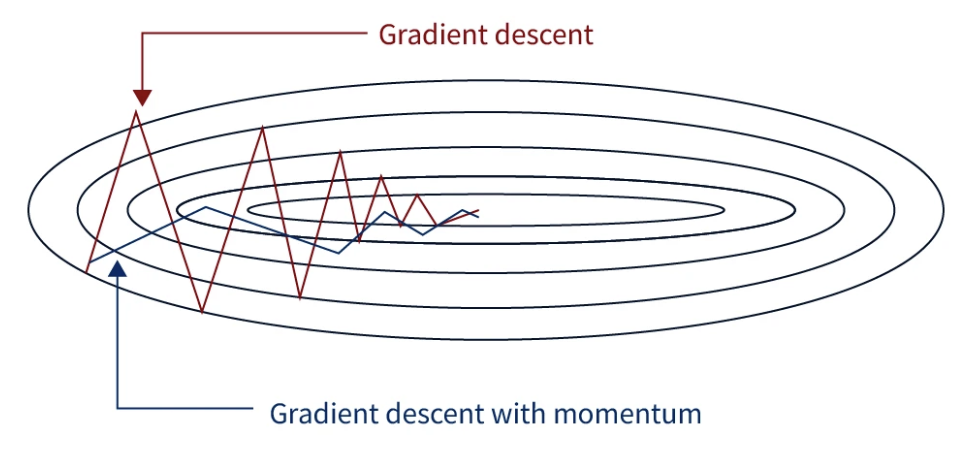
\includegraphics[scale=0.4]{figures/math/stochasticgradientdescent}
\caption{Stochastic Gradient Descent (SGD) Algorithm with and without Momentum}
\end{figure}

\begin{remark} \hlt{Nesterov Momentum}\\
Inspired by Nesterov's accelerated gradient method, the update rules are:
\begin{align}
\bm{v} &\leftarrow \alpha \bm{v} - \epsilon \nabla_{\bm{\theta}} \left(\frac{1}{m} \sum\limits_{i=1}^m L(\bm{f}(\bm{x}^{(i)}; \bm{\theta} + \alpha \bm{v}), \bm{y}^{(i)}) \right) \nonumber \\
\bm{\theta} &\leftarrow \bm{\theta} + \bm{v} \nonumber
\end{align}
Note, gradient is evaluated after current velocity is applied.
\end{remark}

\begin{breakablealgorithm}
\caption{Stochastic Gradient Descent (SGD) with Nesterov Momentum}
\begin{algorithmic}
\Require \\
Learning rate $\epsilon_k$\\
Momentum parameter $\alpha$\\
Initial parameter $\bm{\theta}$\\
Initial velocity $\bm{v}$\\

\While {stopping criterion not met}
\State Sample a minibatch of $m$ samples from the training set $\{\bm{x}^{(1)}, \ldots, \bm{x}^{(m)} \}$ with targets $\bm{y}^{(i)}$
\State Apply interim update: $\tilde{\bm{\theta}} \leftarrow \bm{\theta} + \alpha \bm{v}$
\State Compute gradient (at interim point): $\bm{g} \leftarrow \frac{1}{m} \nabla_{\tilde{\bm{\theta}}} \sum_{i} L(f(\bm{x}^{(i)}; \tilde{\bm{\theta}}), \bm{y}^{(i)})$
\State Compute velocity update: $\bm{v} \leftarrow \alpha \bm{v} - \epsilon \bm{g}$
\State Apply update: $\bm{\theta} \leftarrow \bm{\theta} + \bm{v}$
\EndWhile
\end{algorithmic}
\end{breakablealgorithm}

\begin{figure}[H]
\centering
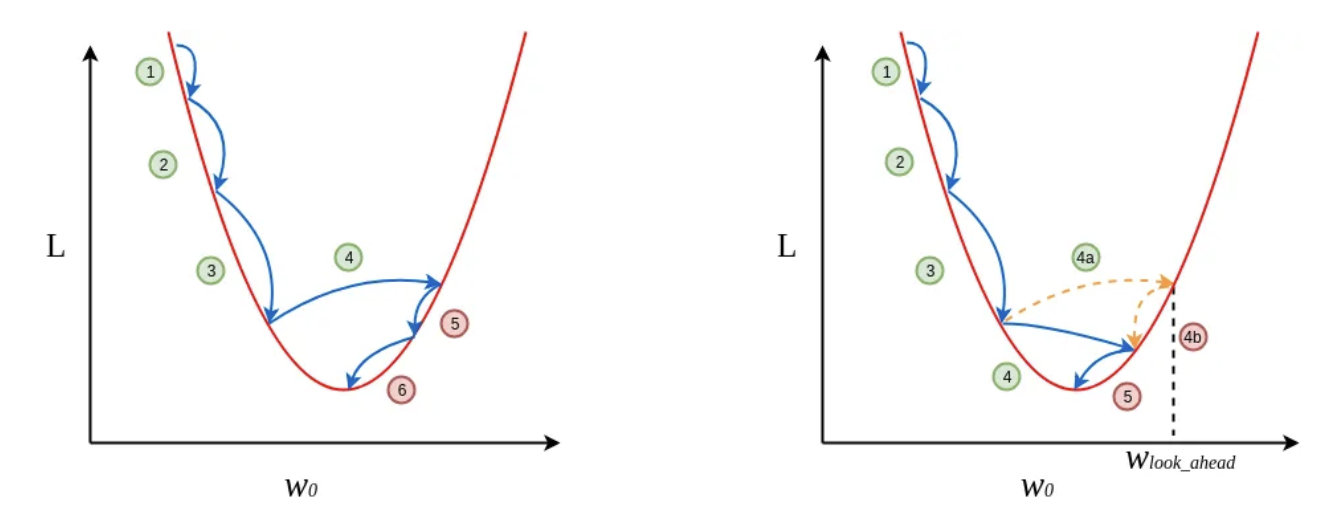
\includegraphics[scale=0.4]{figures/math/nesterov}
\caption{Momentum vs Nesterov Gradient Descent}
\end{figure}


\begin{remark} \hlt{Adaptive Gradient (AdaGrad) Algorithm}\\
Algorithm individually adapts learning rates of all model parameters by scaling them inversely proportional to square root of sum of all of their historical squared values. Has greater progress in more gently sloped directions of parameter space. On deep neural networks, accumulation of squared gradients from beginning of training can result in premature and excessive decrease in effective learning rate.
\end{remark}

\begin{breakablealgorithm}
\caption{Adaptive Gradient (AdaGrad) Algorithm}
\begin{algorithmic}
\Require \\
Global Learning rate $\epsilon$\\
Initial parameter $\bm{\theta}$\\
Small constant $\delta$, perhaps $10^{-7}$ for numerical stability\\

\State Initialise gradient accumulation variable $\bm{r} = \bm{0}$
\While {stopping criterion not met}
\State Sample a minibatch of $m$ samples from the training set $\{\bm{x}^{(1)}, \ldots, \bm{x}^{(m)} \}$ with targets $\bm{y}^{(i)}$
\State Compute gradient: $\bm{g} \leftarrow \frac{1}{m} \nabla_{\bm{\theta}} \sum_i L(f(\bm{x}^{(i)}; \bm{\theta}), \bm{y}^{(i)})$
\State Accumulate squared gradient: $\bm{r} \leftarrow \bm{r} + \bm{g} \odot \bm{g}$
\State Compute update: $\Delta \bm{\theta} \leftarrow - \frac{\epsilon}{\delta + \sqrt{\bm{r}}} \odot \bm{g}$ (Division and square root applied element-wise)
\State Apply update: $\bm{\theta} \leftarrow \bm{\theta} + \Delta \bm{\theta}$
\EndWhile
\end{algorithmic}
\end{breakablealgorithm}

\begin{remark} \hlt{Root Mean Squared Propagation (RMSProp) Algorithm}\\
Modifies AdaGrad to perform better in non-convex setting by changing gradient accumulation into exponentially weighted moving average. RMSProp is effective and practical for deep neural networks.
\end{remark}

\begin{breakablealgorithm}
\caption{Root Mean Squared Propagation (RMSProp) Algorithm}
\begin{algorithmic}
\Require \\
Global Learning rate $\epsilon$\\
Decay rate $\rho$\\
Initial parameter $\bm{\theta}$\\
Small constant $\delta$, perhaps $10^{-6}$ to stabilise division by small numbers\\

\State Initialise accumulation variable $\bm{r} = \bm{0}$
\While {stopping criterion not met}
\State Sample a minibatch of $m$ samples from the training set $\{\bm{x}^{(1)}, \ldots, \bm{x}^{(m)} \}$ with targets $\bm{y}^{(i)}$
\State Compute gradient: $\bm{g} \leftarrow \frac{1}{m} \nabla_{\bm{\theta}} \sum_i L(f(\bm{x}^{(i)}; \bm{\theta}), \bm{y}^{(i)})$
\State Accumulate squared gradient: $\bm{r} \leftarrow \rho \bm{r} + (1 - \rho) \bm{g} \odot \bm{g}$
\State Compute update: $\Delta \bm{\theta} \leftarrow - \frac{\epsilon}{\sqrt{\delta + \bm{r}}} \odot \bm{g}$ ($\frac{\epsilon}{\sqrt{\delta + \bm{r}}}$ applied element-wise)
\State Apply update: $\bm{\theta} \leftarrow \bm{\theta} + \Delta \bm{\theta}$
\EndWhile
\end{algorithmic}
\end{breakablealgorithm}

\begin{breakablealgorithm}
\caption{Root Mean Squared Propagation (RMSProp) Algorithm}
\begin{algorithmic}
\Require \\
Global Learning rate $\epsilon$\\
Decay rate $\rho$\\
Momentum coefficient $\alpha$\\
Initial parameter $\bm{\theta}$\\
Initial velocity $\bm{v}$\\

\State Initialise accumulation variable $\bm{r} = \bm{0}$
\While {stopping criterion not met}
\State Sample a minibatch of $m$ samples from the training set $\{\bm{x}^{(1)}, \ldots, \bm{x}^{(m)} \}$ with targets $\bm{y}^{(i)}$
\State Compute interim update $\tilde{\bm{\theta}} \leftarrow \bm{\theta} + \alpha \bm{v}$
\State Compute gradient: $\bm{g} \leftarrow \frac{1}{m} \nabla_{\tilde{\bm{\theta}}} \sum_i L(f(\bm{x}^{(i)}; \tilde{\bm{\theta}}), \bm{y}^{(i)})$
\State Accumulate gradient: $\bm{r} \leftarrow \rho \bm{r} + (1 - \rho) \bm{g} \odot \bm{g}$
\State Compute velocity update: $\bm{v} \leftarrow \alpha \bm{v} - \frac{\epsilon}{\sqrt{\bm{r}}} \odot \bm{g}$ ($\frac{1}{\sqrt{\bm{r}}}$ applied element-wise)
\State Apply update: $\bm{\theta} \leftarrow \bm{\theta} + \bm{v}$
\EndWhile
\end{algorithmic}
\end{breakablealgorithm}

\begin{remark} \hlt{Adaptive Moment Estimation (Adam) Algorithm}\\
Variant on combination of RMSProp and momentum. Note, momentum is incorporated directly as an estimate of first order moment of gradient; bias corrections are made to estimates of both first-order moments and second-order moments to account for initialisation at origin.\\
Algorithm is fairly robust to choice of hyper-parameters.
\end{remark}

\begin{breakablealgorithm}
\caption{Adaptive Moment Estimation (Adam) Algorithm}
\begin{algorithmic}
\Require \\
Step size $\epsilon$ (Suggested default: $0.001$)\\
Exponential decay rates for moment estimates $\rho_1, \rho_2$ in $[0,1)$ (Suggested defaults: $0.9$ and $0.999$)\\
Small constant $\delta$ used for numerical stabilisation (Suggested default: $10^{-8}$)\\
Initial parameters $\bm{\theta}$\\

\State Initialise $1$st and $2$nd momentum variables $\bm{s} = \bm{0}$, $\bm{r} = \bm{0}$
\State Initialise time step $t=0$
\While {stopping criterion not met}
\State Sample a minibatch of $m$ samples from the training set $\{\bm{x}^{(1)}, \ldots, \bm{x}^{(m)} \}$ with targets $\bm{y}^{(i)}$
\State Compute gradient: $\bm{g} \leftarrow \frac{1}{m} \nabla_{\bm{\theta}} \sum_i L(f(\bm{x}^{(i)}; \bm{\theta}), \bm{y}^{(i)})$
\State Update time step $t \leftarrow t+1$
\State Update biased first and second moment estimate: $\bm{s} \leftarrow \rho_1 \bm{s} + (1-\rho_1) \bm{g}$ and $\bm{r} \leftarrow \rho_2 \bm{r} + (1-\rho_2) \bm{g} \odot \bm{g}$
\State Correct bias in first and second moment: $\hat{\bm{s}} \leftarrow \frac{\bm{s}}{1 - \rho_1^t}$ and $\hat{\bm{r}} \leftarrow \frac{\bm{r}}{1 - \rho_2^t}$
\State Compute update: $\Delta \bm{\theta} = - \epsilon \frac{\hat{\bm{s}}}{\sqrt{\hat{\bm{r}} + \delta}}$ (Operations applied element-wise)
\State Apply update: $\bm{\theta} \leftarrow \bm{\theta} + \Delta \bm{\theta}$
\EndWhile
\end{algorithmic}
\end{breakablealgorithm}

\begin{remark} \hlt{Newton's Method}\\
Based on second-order Taylor's series approximating $J(\bm{\theta})$ near the point $\bm{\theta}_0$, ignoring higher derivatives
\begin{equation}
J(\bm{\theta}) \approx J(\bm{\theta}_0) + (\bm{\theta} - \bm{\theta}_0)^T \nabla_{\bm{\theta}} J(\bm{\theta}_0) + \frac{1}{2} (\bm{\theta} - \bm{\theta}_0)^T \bm{H}(\bm{\theta} - \bm{\theta}_0) \nonumber
\end{equation}
where $\bm{H}$ is the Hessian of $J$ with respect to $\bm{\theta}$ evaluated at $\bm{\theta}_0$.\\
Solving for critical point will get the Newton parameter update rule
\begin{equation}
\bm{\theta}^{*} = \bm{\theta}_0 - \bm{H}^{-1} \nabla_{\bm{\theta}} J(\bm{\theta}_0) \nonumber
\end{equation}
Note that for deep learning, the surface of objective function is non-convex. Regularising the Hessian will solve many of the issues such as saddle points etc.
\begin{equation}
\bm{\theta}^{*} = \bm{\theta}_0 - [H(f(\bm{\theta}_0)) + \alpha \bm{I}]^{-1} \nabla_{\bm{\theta}} J(\bm{\theta}_0) \nonumber
\end{equation}
Due to requirement for inversion of the $k \times k$ matrix with time complexity $O(k^3)$ at every training iteration, only networks with very small number of parameters may be trained with this method.
\end{remark}

\begin{breakablealgorithm}
\caption{Newton's Method with Objective $J(\bm{\theta}) = \frac{1}{m} \sum_{i=1}^m L(f(\bm{x}^{(i)}; \bm{\theta}), y^{(i)})$}
\begin{algorithmic}
\Require \\
Initial parameter $\bm{\theta}_0$\\
Training set of $m$ examples\\

\While {stopping criterion not met}
\State Compute gradient $\bm{g} \leftarrow \frac{1}{m} \nabla_{\bm{\theta}} \sum_i L(f(\bm{x}^{(i)}; \bm{\theta}), \bm{y}^{(i)})$
\State Compute Hessian: $\bm{H} \leftarrow \frac{1}{m} \nabla_{\bm{\theta}}^2 \sum_i L(f(\bm{x}^{(i)}; \bm{\theta}), \bm{y}^{(i)})$
\State Compute Hessian Inverse: $\bm{H}^{-1}$
\State Compute update: $\Delta \bm{\theta} = - \bm{H}^{-1} \bm{g}$
\State Apply update: $\bm{\theta} \leftarrow \bm{\theta} + \Delta \bm{\theta}$
\EndWhile
\end{algorithmic}
\end{breakablealgorithm}

\begin{remark} \hlt{Conjugate Gradient Method}\\
Method effectively avoids computation of inversion Hessian by descending conjugate directions, which is a search direction conjugate to the previous line search direction (will not undo progress made in that direction).\\
Let current and previous search directions be $\bm{d}_{t}, \bm{d}_{t-1}$. At training iteration $t$, the next search direction $\bm{d}_t$ is
\begin{equation}
\bm{d}_t = \nabla_{\bm{\theta}} J(\bm{\theta}) + \beta_t \bm{d}_{t-1} \nonumber
\end{equation}
note that $\beta_t$ may be computed via Fletcher Reeves:
\begin{equation}
\beta_t = \frac{\nabla_{\bm{\theta}} J(\bm{\theta}_t)^T \nabla_{\bm{\theta}} J(\bm{\theta}_t)}{\nabla_{\bm{\theta}} J(\bm{\theta}_{t-1})^T \nabla_{\bm{\theta}} J(\bm{\theta}_{t-1})} \nonumber
\end{equation}
or may be computed with Polak-Ribiere:
\begin{equation}
\beta_t = \frac{(\nabla_{\bm{\theta}} J(\bm{\theta}_t) - \nabla_{\bm{\theta}} J(\bm{\theta}_{t-1}))^T \nabla_{\bm{\theta}} J(\bm{\theta}_t)}{\nabla_{\bm{\theta}} J(\bm{\theta}_{t-1})^T \nabla_{\bm{\theta}} J(\bm{\theta}_{t-1})} \nonumber
\end{equation}
The non-linear conjugate gradient method is a variation which uses occasional resets where the method is restarted with line search along with the unaltered gradient.
\end{remark}

\begin{breakablealgorithm}
\caption{Conjugate Gradient Method}
\begin{algorithmic}
\Require \\
Initial parameter $\bm{\theta}_0$\\
Training set of $m$ examples\\
Initialise $\bm{\rho}_0 = 0$\\
Initialise $g_0 = 0$\\
Initialise $t = 1$\\

\While {stopping criterion not met}
\State Initialise the gradient $\bm{g}_t = \bm{0}$
\State Compute gradient $\bm{g} \leftarrow \frac{1}{m} \nabla_{\bm{\theta}} \sum_i L(f(\bm{x}^{(i)}; \bm{\theta}), \bm{y}^{(i)})$
\State Compute Polak-Ribiere metric: $\beta_t = \frac{(\bm{g}_t - \bm{g}_{t-1})^T \bm{g}_t}{\bm{g}_{t-1}^T \bm{g}_{t-1}}$
\State (Nonlinear conjugate gradient: optionally reset $\beta_t = 0$, i.e., if $t$ is a multiple of some constant $k$)
\State Compute search direction: $\bm{\rho}_t = -\bm{g}_t + \beta_t \bm{\rho}_{t-1}$
\State Perform line search to find: $\epsilon^{*} = \arg \min_{\epsilon} \frac{1}{m} \sum_{i=1}^m L(f(\bm{x}^{(i)}; \bm{\theta}_t + \epsilon \bm{\rho}_t), \bm{y}^{(i)})$
\State (On truly quadratic cost function, analytically solve for $\epsilon^{*}$)
\State Apply update: $\bm{\theta}_{t+1} = \bm{\theta}_{t} + \epsilon^{\theta} \bm{\rho}_t$
\State Apply time step $t \leftarrow t + 1$
\EndWhile
\end{algorithmic}
\end{breakablealgorithm}

\begin{remark} \hlt{Broyden-Fletcher-Goldfarb-Shanno (BGFS) Algorithm}\\
Similar to conjugate gradient, but uses more direct approach to approximation of newton's update.\\
Method approximate the inverse of hessian $\bm{H}$ with matrix $\bm{M}_t$, iteratively refined by low rank updates to better approximate $\bm{H}^{-1}$. Direction of gradient descent is then determined by $\bm{\rho}_t = \bm{M}_t \bm{g}_t$. Line search is performed in this direction to determine step size $\epsilon^{*}$. Final update of parameter is then $\bm{\theta}_{t+1} = \bm{\theta}_t + \epsilon^{*} \bm{\rho}_{t}$.\\
Note, BGFS store matrix $\bm{M}$ which requires $O(n^2)$ memory, making it impractical for most modern models.
\end{remark}
